\documentclass[11pt, a4paper]{article}

\usepackage[utf8]{inputenc}
\usepackage{geometry}
\geometry{a4paper, margin=2.5cm}
\usepackage{graphicx}
\usepackage{float}
\usepackage{hyperref}
\usepackage{titlesec}
\usepackage{booktabs}
\usepackage{caption}
\usepackage{subcaption}

\title{Techniques for Dynamic Visualization of Time-Varying Flood Data}

\author{
    \textbf{Adam Domoslawski} \\
    Student Number: 12241331 \\
    Vienna University of Technology (TU Wien) \\
    \texttt{e12241331@student.tuwien.ac.at}
}

\date{
    \vspace{1em}
    Interdisciplinary Project in Data Science -- Final Report \\
    Main Supervisor: Dr. Martin Schobben (TU Wien) \\
    Project Mentor: Dipl.-Ing. Thais Sarinho Beham (TU Wien) \\
    Co-Supervisor: Assistant Professor Astrid Weiss (TU Wien) \\
    Domain-Specific Lecture: \textit{120.110 Data Retrieval in Earth Observation}, SS~2025 \\
    \vspace{1em}
    December 2025
}

\begin{document}

\maketitle

% ==============================
% 0. ABSTRACT
% ==============================
\begin{abstract}
This project aims to develop visualizations for the general public of satellite-based flood data from Copernicus Emergency Management Services, focusing on the devastating floods that impacted Pakistan in September 2022. The goal is to effectively communicate the extent, likelihood, and uncertainty of time-varying flood events to non-expert audiences. Methods include a literature review, visualization design, and user evaluation via an online survey, with an emphasis on interpretability and accessibility. At its core, the study compares baseline standard visualizations against new techniques—such as polygon smoothing and binning—to determine how spatial risk data can be made more intuitive.
\end{abstract}

% ==============================
% 1. INTRODUCTION
% ==============================
\section{Introduction}
\label{sec:intro}
The Copernicus Emergency Management Services (CEMS) dataset provided for this project consists of satellite-observed, time-dependent flood data. The geographic focus of this study is the region adjacent to the city of Larkana, in Sindh province, Pakistan, located within the Indus river basin. We examine the flooding events from September 2022, which were part of an abnormal series of rains between April and October 2022. This disaster affected more than 2.1 million people, resulting in an estimated 1,729 casualties and 12,867 injuries. 

Because the extent of flooding varies significantly over time, visualizing these dynamic changes in a way that is easily understandable to a wider audience presents a particular challenge. The raw data output is often too technical for laypersons, highlighting the need for highly accessible map representations.

% ==============================
% 2. PROBLEM STATEMENT
% ==============================
\section{Problem Statement}
\label{sec:problem}
The aim of this project is to develop and propose new visualization techniques that can effectively communicate these time-varying flood events, ensuring that they are accessible to the general public. 

The core research question is: \textbf{How can flood risk be effectively combined and visualized for the general public?}

In the context of this study, \textit{flood risk} is defined as a combination of current and future flood \textbf{likelihood} and \textbf{flood extent}. The \textit{general public} refers to civilians without prior experience in analyzing flood visualizations or formal training in geography, flood monitoring, or data science. These individuals must be able to accurately interpret information regarding flood risks even in unfamiliar regions. 

\subsection{Raw Satellite Data Characteristics}
The raw flood data retrieved from Sentinel-1 Synthetic Aperture Radar (SAR) satellites presents significant challenges for non-expert interpretation. Figure~\ref{fig:raw_likelihood} illustrates the unprocessed likelihood data as provided by the CEMS Global Flood Monitoring system. The visualization displays pixel-level probability values ranging from 0 to 100, where higher values indicate greater confidence that a given area is flooded. Additionally, the dataset includes binary flood extent classifications (flooded vs. not-flooded) derived from the same models, which face similar interpretability challenges for layperson audiences.

\begin{figure}[H]
    \centering
    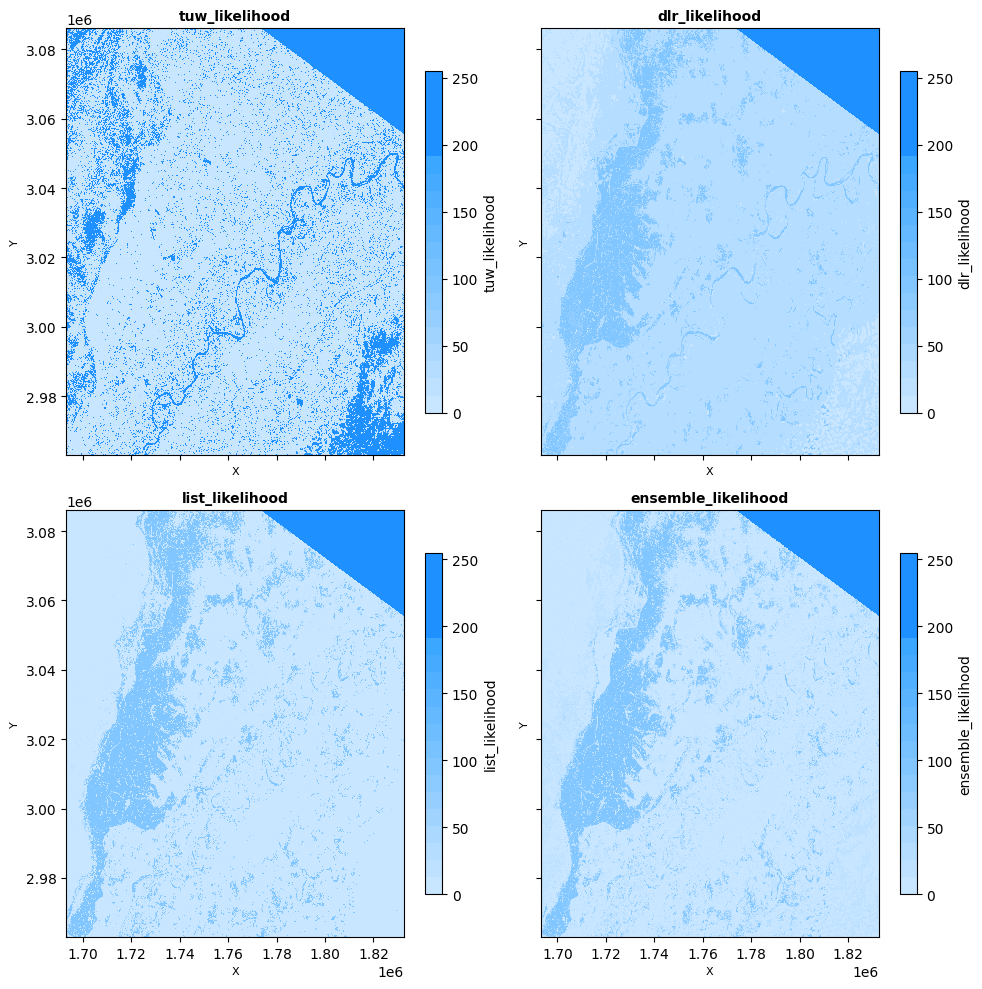
\includegraphics[width=0.75\linewidth]{img/baseline_likelihood_raw.png}
    \caption{Raw flood likelihood data retrieved from Sentinel-1 SAR observations for the Pakistan region (September 2022). The blue color intensity represents the probabilistic confidence of flood detection at each pixel, with brighter blue areas indicating higher likelihood of flooding. The granular, noisy appearance is characteristic of unprocessed satellite radar data.}
    \label{fig:raw_likelihood}
\end{figure}

Several characteristics make this raw data difficult for the general public to interpret:
\begin{itemize}
    \item \textbf{High spatial granularity:} Individual pixels create a fragmented visual appearance that obscures broader flood patterns.
    \item \textbf{Continuous probability scale:} The 0--100 likelihood range requires viewers to mentally categorize risk levels rather than perceiving discrete danger zones.
    \item \textbf{Lack of geographic context:} Without background maps or landmarks, users cannot relate the data to familiar locations or safe routes.
    \item \textbf{Noise and uncertainty:} SAR data inherently contains measurement artifacts and classification uncertainties that appear as visual clutter.
\end{itemize}

These limitations motivate the need for enhanced visualization techniques that preserve critical flood information while significantly improving accessibility and interpretability for non-specialist audiences.

% ==============================
% 3. METHODOLOGY
% ==============================
\section{Methodology}
\label{sec:methods}

\subsection{Literature Research}
To establish a foundation for effective flood visualizations, existing literature on geospatial data representation and interactive mapping tools was reviewed. Rahman and Thakur (2018) propose overlaying flood maps from different timestamps to highlight temporal changes in flood extent, allowing the persistence of flooding to be visualized. A survey by Yussof et al. (2015) emphasizes that utilizing visualization techniques—including technical, interactive, and 3D approaches—can significantly improve user engagement with complex disaster data. 

The challenge of communicating uncertainty in predictions is addressed by Leedal et al. (2010) and Seipel and Lim (2017), who emphasize the importance of visual encodings (like sequential color scales) that convey confidence levels without overwhelming the viewer. Furthermore, recent studies such as Zhu et al. (2025) note that dynamic or simulated views can increase risk cognition for the general public.

\subsection{Data \& Pre-processing}
\label{subsec:data}
This project utilizes the Global Flood Monitoring (GFM) dataset from CEMS, offering flood detection data based on satellite observations for the selected regions in Pakistan. The dataset provides a comprehensive look at flood risk by supplying four distinct versions of flood likelihood and flood extent generated by different models: \texttt{tuw}, \texttt{dlr}, \texttt{lst}, and an \texttt{ensemble} model. 

In addition to the raw model outputs, the dataset includes crucial masking layers necessary for data refinement:
\begin{itemize}
    \item \textbf{Reference Water Mask:} A flag used to identify permanent inland water bodies (such as existing rivers or lakes).
    \item \textbf{Exclusion Mask:} A flag that identifies and excludes areas of the map that were not successfully scanned by the Synthetic Aperture Radar (SAR) satellite.
\end{itemize}

During pre-processing, a pixel was only classified as a valid flooded area if the model output indicated flooding, and it was simultaneously not part of the \texttt{exclusion\_mask} and not flagged by the \texttt{reference\_water\_mask}. Furthermore, spatial dimensions were re-projected to standard longitude and latitude (WGS84) to allow compatibility with geographic basemaps.

\subsection{Comparison of Flood Models}
\label{subsec:model_comparison}
To provide a thorough foundation for the visualization techniques, an initial comparison of the four retrieved model types (\texttt{tuw}, \texttt{dlr}, \texttt{lst}, and \texttt{ensemble}) was conducted. Because each model uses slightly different algorithms and radar interpretations to classify water, their resulting likelihoods and extents vary. Understanding these differences is vital before deciding which base data should be simplified for the general public.

\begin{figure}[H]
    \centering
    % \includegraphics[width=\linewidth]{img/model_comparison.png}
    \caption{Placeholder: A side-by-side comparison of the raw flood extent and likelihood outputs from the tuw, dlr, lst, and ensemble models for the Pakistan 2022 case study.}
    \label{fig:model_comparison}
\end{figure}



\subsection{Visualizations}
To compare interpretability among laypersons, several visualization techniques were implemented.

\begin{enumerate}
    \item \textbf{Baseline (CEMS)}: The default visualization directly plotting raw raster likelihood data.
    \item \textbf{Baseline with Map}: The default visualization overlaid onto a geographic basemap to provide essential spatial context.
    \item \textbf{Polygon (Simplified)}: Smoothing the underlying flood-likelihood raster values into larger, contiguous polygon areas to reduce visual fragmentation and make spatial trends instantly recognizable.
    \item \textbf{Mixed Method}: Combining polygon smoothing with original flood extent raster information, serving as a middle ground between highly smoothed patterns and detailed raster views.
    \item \textbf{Binning-based}: Grouping flood likelihood into discrete categorical risk bins (e.g., Low, Medium, High) with distinct visual encodings, simplifying the continuous value space.
\end{enumerate}

% --- FIGURE PLACEHOLDERS ---
\begin{figure}[H]
    \centering
    % \includegraphics[width=0.8\linewidth]{img/pakistan_baseline_map.png}
    \caption{Placeholder: Baseline visualization overlaid on a background map.}
    \label{fig:baseline_map}
\end{figure}

\begin{figure}[H]
    \centering
    % \includegraphics[width=0.8\linewidth]{img/pakistan_polygon.png}
    \caption{Placeholder: Flood likelihood smoothed with polygons.}
    \label{fig:polygon}
\end{figure}

\begin{figure}[H]
    \centering
    % \includegraphics[width=0.8\linewidth]{img/pakistan_binned.png}
    \caption{Placeholder: Binned flood likelihood representing discrete risk categories.}
    \label{fig:binned}
\end{figure}




% ==============================
% 4. SURVEY
% ==============================
\section{Survey Structure}
\label{sec:survey}
To evaluate the effectiveness of the developed visualizations regarding clarity, interpretability, and accessibility, an online A/B testing survey was conducted using SoSci Survey. The target audience intentionally comprised the general public to test real-world layperson comprehension. 

The survey was divided into three sections:
\begin{itemize}
    \item \textbf{Demographics and Familiarity}: To gauge prior knowledge of geospatial maps, ensuring the sample reflects inexperienced users.
    \item \textbf{Task and Confidence Evaluation}: Participants were shown the various visualizations in randomized order. They were asked simple navigation/safety questions (e.g., assessing the safety of a plotted point) followed by a question rating their confidence in their answer on a Likert scale. 
    \item \textbf{Ranking}: A final review where participants ranked the visualizations from easiest to hardest to interpret via drag-and-drop.
\end{itemize}

Accessibility was also considered. Color schemes were validated using a Color Blindness Simulator (Coblis) to ensure distinguishability across different types of color vision deficiencies.

% ==============================
% 5. RESULTS & DISCUSSION 
% ==============================
\section{Results and Discussion}
\label{sec:results}
\textit{[Note to Author: Insert your own survey analysis here. Describe how the different visualizations performed regarding participant accuracy, user confidence, and final rankings based on your data. Compare the Polygon/Binned visualizations against the Baseline for the Pakistan case study.]}

\section{Conclusion}
\label{sec:conclusion}
\textit{[Note to Author: Summarize the findings based on your survey results. Conclude on which visualization approach best answers the problem statement for the general public.]}

% ==============================
% 6. SUPPLEMENTARY CONSIDERATIONS
% ==============================
\section{Supplementary Considerations (Optional)}
\label{sec:supplementary}
Beyond standard 2D map views, additional approaches were investigated to enhance future flood communication. These included creating gap-free seamless composites using a First-Valid-Pixel temporal mosaic to counteract missing satellite scanning areas. Furthermore, exploring 3D visualizations that combine flood depth with regional terrain elevation presents a promising avenue for helping decision-makers and the public immediately identify safe, elevated zones compared to at-risk lowlands.

% ==============================
% 7. BIBLIOGRAPHY
% ==============================
\begin{thebibliography}{10}

\bibitem{Leedal2010}
D.~T. Leedal, K.~J. Beven, and P.~C. Young.
\newblock Communicating uncertainty in river stage forecasts.
\newblock {\em Hydrology and Earth System Sciences}, 14:957--968, 2010.

\bibitem{Rahman2018}
M.~R. Rahman and P.~K. Thakur.
\newblock Detecting, mapping and analysing of flood water propagation using synthetic aperture radar (SAR) satellite data and GIS: A case study from the Kendrapara district of Orissa state of India.
\newblock {\em The Egyptian Journal of Remote Sensing and Space Science}, 21:S37--S41, 2018.

\bibitem{Seipel2017}
S.~Seipel and N.~J. Lim.
\newblock Visualizing uncertainty in flood inundation maps.
\newblock {\em International Journal of Geographical Information Science}, 31(10):2018--2039, 2017.

\bibitem{Yussof2015}
S.~Yussof, N.~Husin, Z.~Ibrahim, A.~Ghapar, N.~Din, and F.~Abdullah.
\newblock Review of visualization techniques for landslide and flood disaster data.
\newblock {\em Research Journal of Applied Sciences, Engineering and Technology}, 9:700--705, 2015.

\bibitem{Zhu2025}
J.~Zhu, D.~F. Laefer, R.~P. Lejano, P.~Gmelch, E.~O'Keeffe, and K.~Chandna.
\newblock From 2D to 3D: Flood risk communication in a flood-prone neighborhood via dynamic, isometric street views.
\newblock {\em Progress in Disaster Science}, 26:100419, 2025.

\bibitem{Cohen2017}
S.~Cohen, et al. 
\newblock Estimating floodwater depths from flood inundation maps and topography.
\newblock {\em JAWRA Journal of the American Water Resources Association}, 54, 2017.

\end{thebibliography}

\end{document}